\section{Introduction}
% \IEEEPARstart{T}{his} file
\IEEEPARstart{V}{ideo} captioning requires generating coherent natural-language descriptions from dynamic visual content, demanding simultaneous understanding of spatial appearance, temporal dynamics, and their alignment with language. Owing to its broad applications in video retrieval, human–computer interaction, and assistive technologies, the task has attracted sustained research interest. Existing approaches have evolved from early template-based systems \cite{khanDescribingVideoContents2012, guadarramaYouTube2TextRecognizingDescribing2013} and CNN–RNN encoder–decoder frameworks \cite{yaoDescribingVideosExploiting2015, venugopalanSequenceSequenceVideo2015} to Transformer-based architectures \cite{zhouEndtoEndDenseVideo2018,chenTVTTwoViewTransformer2018}, which have become the dominant paradigm due to their superior sequence modeling capability.

Despite their success, recent Transformer-based video captioning methods commonly exhibit two architectural tendencies that warrant closer examination. First, most approaches introduce substantial intermediate processing before caption generation. Extracted visual features are typically refined through stacked encoder layers, multimodal fusion modules, or external knowledge graph pipelines before reaching the decoder. While these components can improve representation quality, they also increase architectural complexity, computational cost, and susceptibility to error propagation from intermediate predictors. Second, caption generation is usually formulated as a strictly left-to-right (L2R) autoregressive process, preventing the model from exploiting future linguistic context during decoding.

\begin{figure}[!t]
\centering
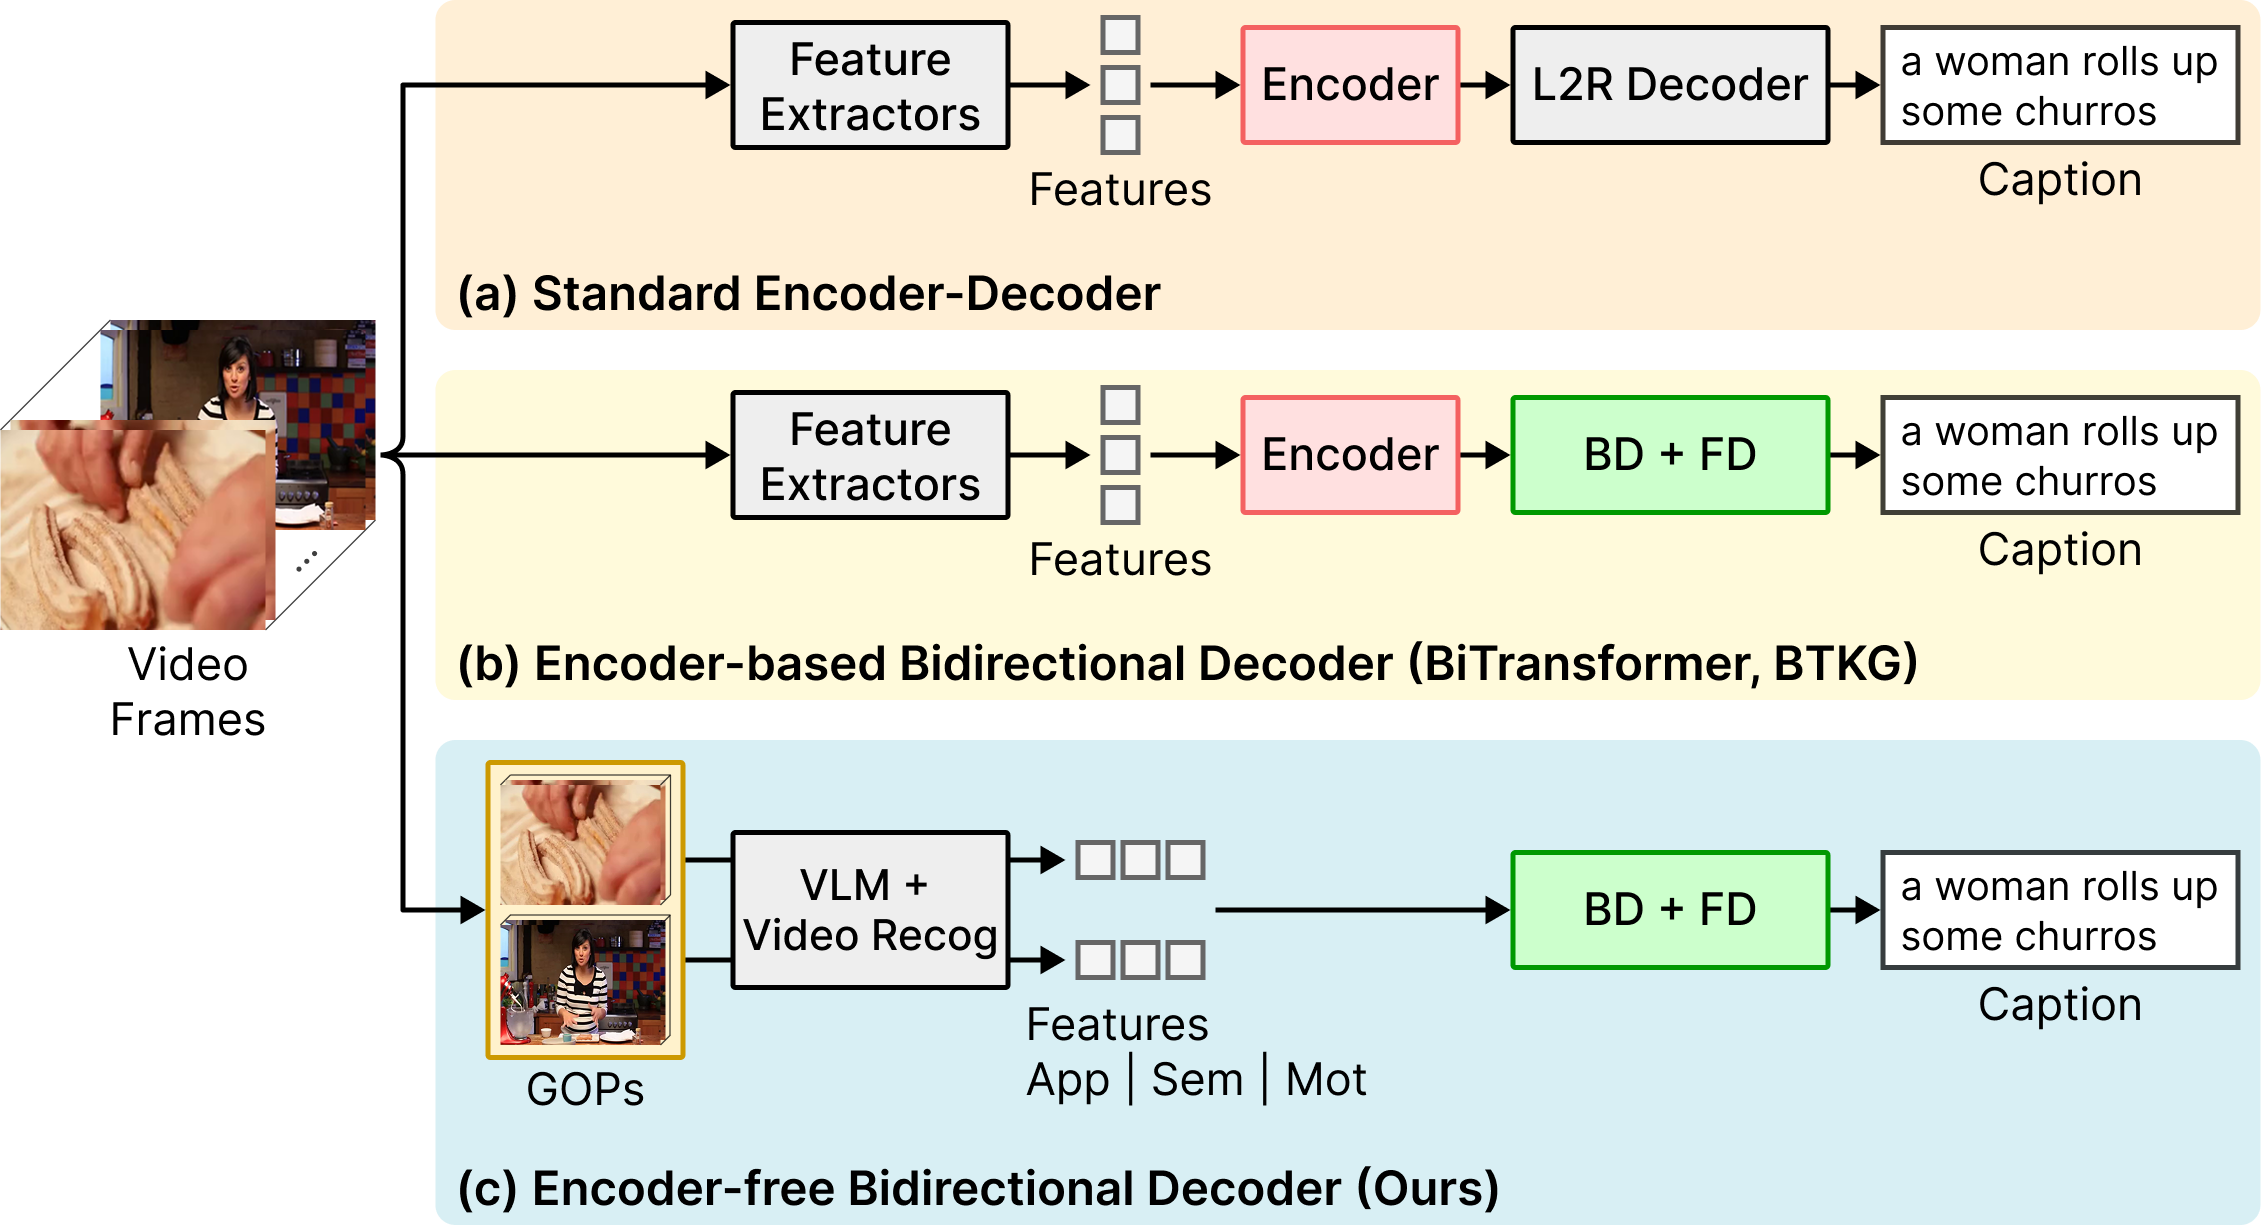
\includegraphics[width=\columnwidth]{figures/fig01_architecture_comparison.png}
\caption{Comparison of three architectural paradigms in Transformer-based video captioning. (a) Standard encoder-decoder: features are refined through intermediate encoding before left-to-right decoding. (b) Encoder-based bidirectional decoder: features are processed through intermediate encoder(s) before reaching the backward (BD) and forward (FD) decoders. (c) Encoder-free bidirectional decoder (proposed): features are projected directly into the bidirectional decoder system without intermediate encoding.}
\label{fig:fig01_architecture_comparison}
\end{figure}

These design choices are increasingly worth revisiting given advances in large-scale pre-trained models. Modern vision-language and video recognition models already provide semantically rich and well-structured representations, raising the question of whether additional intermediate encoding stages continue to provide proportional benefits or merely introduce redundant processing overhead. Meanwhile, bidirectional decoding strategies, where reverse-direction context supplements standard L2R generation, have demonstrated improvements in caption coherence \cite{zhongBiTransformerAugmentingSemantic2022, zhongBidirectionalTransformerKnowledge2024}. However, existing bidirectional approaches still rely on intermediate encoders to process extracted features, inheriting the same architectural and computational burdens. Consequently, the combination of encoder-free multimodal integration and bidirectional autoregressive decoding remains unexplored in video captioning. Fig.~\ref{fig:fig01_architecture_comparison} contrasts these architectural paradigms and situates the proposed approach relative to existing designs.

Motivated by these observations, we propose the Encoder-free Bidirectional Decoder Transformer (BiDecT), a video captioning framework that integrates multimodal representations into a bidirectional decoding architecture without any intermediate encoding stage. To reduce redundant frame-level processing, each video is represented as a sequence of Groups of Pictures (GOPs). From each GOP, the model extracts three complementary modalities: appearance features from a pre-trained vision-language model, semantic features derived from its generated frame-level descriptions, and motion features that capture short-term temporal dynamics. A lightweight embedding module with modality-specific type embeddings projects these features into a shared representation space before they are fed into the decoder system. The decoding architecture consists of a backward decoder that generates a reverse caption to construct a global backward context, and a forward decoder that conditions on both the multimodal representation and this context to produce the final caption. During training, a pseudo reverse caption strategy is adopted to prevent information leakage between the two decoding directions.

Our main contributions are as follows:
\begin{itemize}
\item We propose BiDecT, an encoder-free video captioning framework that directly integrates multimodal representations into a bidirectional decoding architecture. To the best of our knowledge, this is the first approach in video captioning to combine encoder-free multimodal integration with bidirectional autoregressive decoding.
\item We design a GOP-based multimodal feature extraction pipeline that derives appearance, semantic, and motion representations from structured video segments, exploiting intra-segment temporal coherence while reducing redundant frame-level processing.
\item We introduce a dual-purpose feature extraction scheme that leverages a pre-trained vision-language model for both appearance and semantic feature extraction. This design transfers both visual and linguistic knowledge from image captioning to video captioning without relying on explicit knowledge graph construction.
\item Extensive experiments on MSVD, MSR-VTT, and VATEX demonstrate that BiDecT achieves state-of-the-art CIDEr scores of 138.0, 64.8, and 78.2, outperforming prior leading methods by 10.8, 2.8, and 5.2 points, respectively, while reducing per-epoch training time by up to 42.7\% compared to encoder-based variants.
\end{itemize}

% ==== TODO: Omit the paper outline to save space ====
% The remainder of this paper is organized as follows. Section~\ref{sec:02_rw} reviews related work. Section~\ref{sec:03_background} introduces the GOP structure and the Transformer building blocks underlying the proposed model. Section~\ref{sec:04_method} presents the proposed BiDecT architecture in detail. Section~\ref{sec:05_exp} reports experimental results, including comparisons with state-of-the-art methods, hyperparameter analysis, and ablation studies. Finally, Section~\ref{sec:06_con} concludes the paper.
